\documentclass[twoside]{book}

% Packages required by doxygen
\usepackage{fixltx2e}
\usepackage{calc}
\usepackage{doxygen}
\usepackage[export]{adjustbox} % also loads graphicx
\usepackage{graphicx}
\usepackage[utf8]{inputenc}
\usepackage{makeidx}
\usepackage{multicol}
\usepackage{multirow}
\PassOptionsToPackage{warn}{textcomp}
\usepackage{textcomp}
\usepackage[nointegrals]{wasysym}
\usepackage[table]{xcolor}

% Font selection
\usepackage[T1]{fontenc}
\usepackage[scaled=.90]{helvet}
\usepackage{courier}
\usepackage{amssymb}
\usepackage{sectsty}
\renewcommand{\familydefault}{\sfdefault}
\allsectionsfont{%
  \fontseries{bc}\selectfont%
  \color{darkgray}%
}
\renewcommand{\DoxyLabelFont}{%
  \fontseries{bc}\selectfont%
  \color{darkgray}%
}
\newcommand{\+}{\discretionary{\mbox{\scriptsize$\hookleftarrow$}}{}{}}

% Page & text layout
\usepackage{geometry}
\geometry{%
  a4paper,%
  top=2.5cm,%
  bottom=2.5cm,%
  left=2.5cm,%
  right=2.5cm%
}
\tolerance=750
\hfuzz=15pt
\hbadness=750
\setlength{\emergencystretch}{15pt}
\setlength{\parindent}{0cm}
\setlength{\parskip}{3ex plus 2ex minus 2ex}
\makeatletter
\renewcommand{\paragraph}{%
  \@startsection{paragraph}{4}{0ex}{-1.0ex}{1.0ex}{%
    \normalfont\normalsize\bfseries\SS@parafont%
  }%
}
\renewcommand{\subparagraph}{%
  \@startsection{subparagraph}{5}{0ex}{-1.0ex}{1.0ex}{%
    \normalfont\normalsize\bfseries\SS@subparafont%
  }%
}
\makeatother

% Headers & footers
\usepackage{fancyhdr}
\pagestyle{fancyplain}
\fancyhead[LE]{\fancyplain{}{\bfseries\thepage}}
\fancyhead[CE]{\fancyplain{}{}}
\fancyhead[RE]{\fancyplain{}{\bfseries\leftmark}}
\fancyhead[LO]{\fancyplain{}{\bfseries\rightmark}}
\fancyhead[CO]{\fancyplain{}{}}
\fancyhead[RO]{\fancyplain{}{\bfseries\thepage}}
\fancyfoot[LE]{\fancyplain{}{}}
\fancyfoot[CE]{\fancyplain{}{}}
\fancyfoot[RE]{\fancyplain{}{\bfseries\scriptsize Generated by Doxygen }}
\fancyfoot[LO]{\fancyplain{}{\bfseries\scriptsize Generated by Doxygen }}
\fancyfoot[CO]{\fancyplain{}{}}
\fancyfoot[RO]{\fancyplain{}{}}
\renewcommand{\footrulewidth}{0.4pt}
\renewcommand{\chaptermark}[1]{%
  \markboth{#1}{}%
}
\renewcommand{\sectionmark}[1]{%
  \markright{\thesection\ #1}%
}

% Indices & bibliography
\usepackage{natbib}
\usepackage[titles]{tocloft}
\setcounter{tocdepth}{3}
\setcounter{secnumdepth}{5}
\makeindex

% Hyperlinks (required, but should be loaded last)
\usepackage{ifpdf}
\ifpdf
  \usepackage[pdftex,pagebackref=true]{hyperref}
\else
  \usepackage[ps2pdf,pagebackref=true]{hyperref}
\fi
\hypersetup{%
  colorlinks=true,%
  linkcolor=blue,%
  citecolor=blue,%
  unicode%
}

% Custom commands
\newcommand{\clearemptydoublepage}{%
  \newpage{\pagestyle{empty}\cleardoublepage}%
}

\usepackage{caption}
\captionsetup{labelsep=space,justification=centering,font={bf},singlelinecheck=off,skip=4pt,position=top}

%===== C O N T E N T S =====

\begin{document}

% Titlepage & ToC
\hypersetup{pageanchor=false,
             bookmarksnumbered=true,
             pdfencoding=unicode
            }
\pagenumbering{alph}
\begin{titlepage}
\vspace*{7cm}
\begin{center}%
{\Large My Project }\\
\vspace*{1cm}
{\large Generated by Doxygen 1.8.12}\\
\end{center}
\end{titlepage}
\clearemptydoublepage
\pagenumbering{roman}
\tableofcontents
\clearemptydoublepage
\pagenumbering{arabic}
\hypersetup{pageanchor=true}

%--- Begin generated contents ---
\chapter{Hierarchical Index}
\section{Class Hierarchy}
This inheritance list is sorted roughly, but not completely, alphabetically\+:\begin{DoxyCompactList}
\item \contentsline{section}{ch.\+bbc.\+partyplanner.\+controller.\+Cookie\+Helper}{\pageref{classch_1_1bbc_1_1partyplanner_1_1controller_1_1_cookie_helper}}{}
\item Serializable\begin{DoxyCompactList}
\item \contentsline{section}{ch.\+bbc.\+partyplanner.\+controller.\+Event\+Controller}{\pageref{classch_1_1bbc_1_1partyplanner_1_1controller_1_1_event_controller}}{}
\item \contentsline{section}{ch.\+bbc.\+partyplanner.\+controller.\+Event\+View\+Controller}{\pageref{classch_1_1bbc_1_1partyplanner_1_1controller_1_1_event_view_controller}}{}
\item \contentsline{section}{ch.\+bbc.\+partyplanner.\+controller.\+User\+Controller}{\pageref{classch_1_1bbc_1_1partyplanner_1_1controller_1_1_user_controller}}{}
\end{DoxyCompactList}
\end{DoxyCompactList}

\chapter{Class Index}
\section{Class List}
Here are the classes, structs, unions and interfaces with brief descriptions\+:\begin{DoxyCompactList}
\item\contentsline{section}{\hyperlink{classch_1_1bbc_1_1partyplanner_1_1controller_1_1_cookie_helper}{ch.\+bbc.\+partyplanner.\+controller.\+Cookie\+Helper} }{\pageref{classch_1_1bbc_1_1partyplanner_1_1controller_1_1_cookie_helper}}{}
\item\contentsline{section}{\hyperlink{classch_1_1bbc_1_1partyplanner_1_1controller_1_1_event_controller}{ch.\+bbc.\+partyplanner.\+controller.\+Event\+Controller} }{\pageref{classch_1_1bbc_1_1partyplanner_1_1controller_1_1_event_controller}}{}
\item\contentsline{section}{\hyperlink{classch_1_1bbc_1_1partyplanner_1_1controller_1_1_event_view_controller}{ch.\+bbc.\+partyplanner.\+controller.\+Event\+View\+Controller} }{\pageref{classch_1_1bbc_1_1partyplanner_1_1controller_1_1_event_view_controller}}{}
\item\contentsline{section}{\hyperlink{classch_1_1bbc_1_1partyplanner_1_1controller_1_1_user_controller}{ch.\+bbc.\+partyplanner.\+controller.\+User\+Controller} }{\pageref{classch_1_1bbc_1_1partyplanner_1_1controller_1_1_user_controller}}{}
\end{DoxyCompactList}

\chapter{Class Documentation}
\hypertarget{classch_1_1bbc_1_1partyplanner_1_1controller_1_1_cookie_helper}{}\section{ch.\+bbc.\+partyplanner.\+controller.\+Cookie\+Helper Class Reference}
\label{classch_1_1bbc_1_1partyplanner_1_1controller_1_1_cookie_helper}\index{ch.\+bbc.\+partyplanner.\+controller.\+Cookie\+Helper@{ch.\+bbc.\+partyplanner.\+controller.\+Cookie\+Helper}}
\subsection*{Public Member Functions}
\begin{DoxyCompactItemize}
\item 
\hypertarget{classch_1_1bbc_1_1partyplanner_1_1controller_1_1_cookie_helper_a4f1561a00451ec1b947d8da83748a1a9}{}\label{classch_1_1bbc_1_1partyplanner_1_1controller_1_1_cookie_helper_a4f1561a00451ec1b947d8da83748a1a9} 
void {\bfseries set\+Logged\+In\+Cookie} (String user\+Id, int expiry, Faces\+Context faces\+Context)
\item 
\hypertarget{classch_1_1bbc_1_1partyplanner_1_1controller_1_1_cookie_helper_a64f4b3a2b843adb1ddb3f3b4354bf8c4}{}\label{classch_1_1bbc_1_1partyplanner_1_1controller_1_1_cookie_helper_a64f4b3a2b843adb1ddb3f3b4354bf8c4} 
int {\bfseries get\+User\+Id\+Cookie} (Faces\+Context faces\+Context)
\end{DoxyCompactItemize}


The documentation for this class was generated from the following file\+:\begin{DoxyCompactItemize}
\item 
Cookie\+Helper.\+java\end{DoxyCompactItemize}

\hypertarget{classch_1_1bbc_1_1partyplanner_1_1controller_1_1_event_controller}{}\section{ch.\+bbc.\+partyplanner.\+controller.\+Event\+Controller Class Reference}
\label{classch_1_1bbc_1_1partyplanner_1_1controller_1_1_event_controller}\index{ch.\+bbc.\+partyplanner.\+controller.\+Event\+Controller@{ch.\+bbc.\+partyplanner.\+controller.\+Event\+Controller}}
Inheritance diagram for ch.\+bbc.\+partyplanner.\+controller.\+Event\+Controller\+:\begin{figure}[H]
\begin{center}
\leavevmode
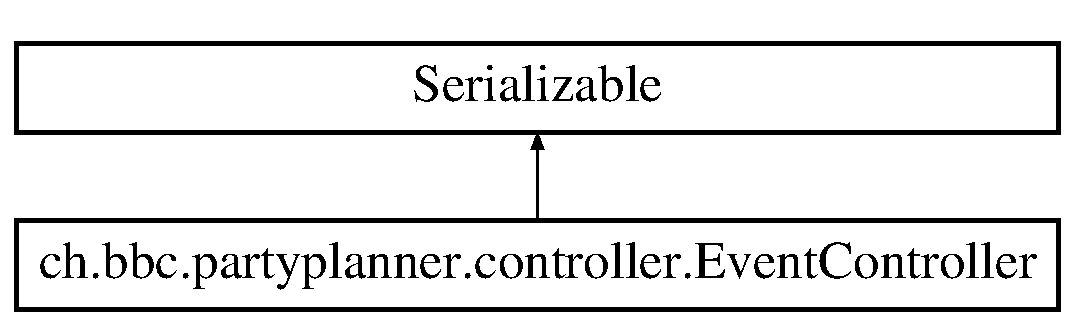
\includegraphics[height=2.000000cm]{classch_1_1bbc_1_1partyplanner_1_1controller_1_1_event_controller}
\end{center}
\end{figure}
\subsection*{Public Member Functions}
\begin{DoxyCompactItemize}
\item 
\hypertarget{classch_1_1bbc_1_1partyplanner_1_1controller_1_1_event_controller_ac32d1ed6c79fc8eed2b84489f840cc43}{}\label{classch_1_1bbc_1_1partyplanner_1_1controller_1_1_event_controller_ac32d1ed6c79fc8eed2b84489f840cc43} 
void {\bfseries init} ()
\item 
\hypertarget{classch_1_1bbc_1_1partyplanner_1_1controller_1_1_event_controller_afac788cb2a726f80c8885987ba834c3d}{}\label{classch_1_1bbc_1_1partyplanner_1_1controller_1_1_event_controller_afac788cb2a726f80c8885987ba834c3d} 
String {\bfseries go\+To\+Event} ()
\item 
\hypertarget{classch_1_1bbc_1_1partyplanner_1_1controller_1_1_event_controller_a19d6480876414753f37eb7a95062e2f3}{}\label{classch_1_1bbc_1_1partyplanner_1_1controller_1_1_event_controller_a19d6480876414753f37eb7a95062e2f3} 
String {\bfseries create} ()
\item 
\hypertarget{classch_1_1bbc_1_1partyplanner_1_1controller_1_1_event_controller_ad36557d04ac8036dbc8958d8ebc68695}{}\label{classch_1_1bbc_1_1partyplanner_1_1controller_1_1_event_controller_ad36557d04ac8036dbc8958d8ebc68695} 
String {\bfseries take\+Me\+Home} ()
\item 
\hypertarget{classch_1_1bbc_1_1partyplanner_1_1controller_1_1_event_controller_a407ec50a7ea48c307545ca3e6bb22b03}{}\label{classch_1_1bbc_1_1partyplanner_1_1controller_1_1_event_controller_a407ec50a7ea48c307545ca3e6bb22b03} 
String {\bfseries generate\+Event\+Adress} ()
\item 
\hypertarget{classch_1_1bbc_1_1partyplanner_1_1controller_1_1_event_controller_a8c5dbd966470309a13e13d2679e38604}{}\label{classch_1_1bbc_1_1partyplanner_1_1controller_1_1_event_controller_a8c5dbd966470309a13e13d2679e38604} 
void {\bfseries save\+New\+Products} ()
\item 
\hypertarget{classch_1_1bbc_1_1partyplanner_1_1controller_1_1_event_controller_a8946a84f79ea5adbba767a411227df23}{}\label{classch_1_1bbc_1_1partyplanner_1_1controller_1_1_event_controller_a8946a84f79ea5adbba767a411227df23} 
String {\bfseries delete\+By\+Id} ()
\item 
\hypertarget{classch_1_1bbc_1_1partyplanner_1_1controller_1_1_event_controller_a70531498534f3663c5c1aff011b1143a}{}\label{classch_1_1bbc_1_1partyplanner_1_1controller_1_1_event_controller_a70531498534f3663c5c1aff011b1143a} 
boolean {\bfseries is\+Search\+Status} ()
\item 
\hypertarget{classch_1_1bbc_1_1partyplanner_1_1controller_1_1_event_controller_aa7830340192ca6afd3e00dbb02609d3a}{}\label{classch_1_1bbc_1_1partyplanner_1_1controller_1_1_event_controller_aa7830340192ca6afd3e00dbb02609d3a} 
void {\bfseries set\+Search\+Status} (boolean search\+Status)
\item 
\hypertarget{classch_1_1bbc_1_1partyplanner_1_1controller_1_1_event_controller_a8f4136df7c80cf01441cd54baf1347ac}{}\label{classch_1_1bbc_1_1partyplanner_1_1controller_1_1_event_controller_a8f4136df7c80cf01441cd54baf1347ac} 
Event {\bfseries get\+Event} ()
\item 
\hypertarget{classch_1_1bbc_1_1partyplanner_1_1controller_1_1_event_controller_afaee5fc8b9ce1f8d082e64b8ee3b8e0f}{}\label{classch_1_1bbc_1_1partyplanner_1_1controller_1_1_event_controller_afaee5fc8b9ce1f8d082e64b8ee3b8e0f} 
void {\bfseries set\+Event} (Event event)
\item 
\hypertarget{classch_1_1bbc_1_1partyplanner_1_1controller_1_1_event_controller_a93c86b4767cf42bbfc70989884a61323}{}\label{classch_1_1bbc_1_1partyplanner_1_1controller_1_1_event_controller_a93c86b4767cf42bbfc70989884a61323} 
String {\bfseries get\+Requested\+Event} ()
\item 
\hypertarget{classch_1_1bbc_1_1partyplanner_1_1controller_1_1_event_controller_a812455a40886d584c213627a4915d1af}{}\label{classch_1_1bbc_1_1partyplanner_1_1controller_1_1_event_controller_a812455a40886d584c213627a4915d1af} 
void {\bfseries set\+Requested\+Event} (String requested\+Event)
\item 
\hypertarget{classch_1_1bbc_1_1partyplanner_1_1controller_1_1_event_controller_a498d5deac47eca5d05c6c1d58d4182a0}{}\label{classch_1_1bbc_1_1partyplanner_1_1controller_1_1_event_controller_a498d5deac47eca5d05c6c1d58d4182a0} 
List$<$ Event $>$ {\bfseries get\+All\+Events} ()
\item 
\hypertarget{classch_1_1bbc_1_1partyplanner_1_1controller_1_1_event_controller_aa8e437aa4cd1273fac16f77c17dc7d55}{}\label{classch_1_1bbc_1_1partyplanner_1_1controller_1_1_event_controller_aa8e437aa4cd1273fac16f77c17dc7d55} 
void {\bfseries set\+All\+Events} (List$<$ Event $>$ all\+Events)
\item 
\hypertarget{classch_1_1bbc_1_1partyplanner_1_1controller_1_1_event_controller_ada0f32993d0e75fd9d6fc03036299b44}{}\label{classch_1_1bbc_1_1partyplanner_1_1controller_1_1_event_controller_ada0f32993d0e75fd9d6fc03036299b44} 
\hyperlink{classch_1_1bbc_1_1partyplanner_1_1controller_1_1_user_controller}{User\+Controller} {\bfseries get\+User\+Controller} ()
\item 
\hypertarget{classch_1_1bbc_1_1partyplanner_1_1controller_1_1_event_controller_a99ee5c29f22bc5bdce54d8a4728652e8}{}\label{classch_1_1bbc_1_1partyplanner_1_1controller_1_1_event_controller_a99ee5c29f22bc5bdce54d8a4728652e8} 
void {\bfseries set\+User\+Controller} (\hyperlink{classch_1_1bbc_1_1partyplanner_1_1controller_1_1_user_controller}{User\+Controller} user\+Controller)
\item 
\hypertarget{classch_1_1bbc_1_1partyplanner_1_1controller_1_1_event_controller_abacda5c9bf09877a6ea39a012316b362}{}\label{classch_1_1bbc_1_1partyplanner_1_1controller_1_1_event_controller_abacda5c9bf09877a6ea39a012316b362} 
int {\bfseries get\+Current\+Event\+Id} ()
\item 
\hypertarget{classch_1_1bbc_1_1partyplanner_1_1controller_1_1_event_controller_aa0a2431cd4dafe295f6340b719aacd38}{}\label{classch_1_1bbc_1_1partyplanner_1_1controller_1_1_event_controller_aa0a2431cd4dafe295f6340b719aacd38} 
void {\bfseries set\+Current\+Event\+Id} (int current\+Event\+Id)
\end{DoxyCompactItemize}


The documentation for this class was generated from the following file\+:\begin{DoxyCompactItemize}
\item 
Event\+Controller.\+java\end{DoxyCompactItemize}

\hypertarget{classch_1_1bbc_1_1partyplanner_1_1controller_1_1_event_view_controller}{}\section{ch.\+bbc.\+partyplanner.\+controller.\+Event\+View\+Controller Class Reference}
\label{classch_1_1bbc_1_1partyplanner_1_1controller_1_1_event_view_controller}\index{ch.\+bbc.\+partyplanner.\+controller.\+Event\+View\+Controller@{ch.\+bbc.\+partyplanner.\+controller.\+Event\+View\+Controller}}
Inheritance diagram for ch.\+bbc.\+partyplanner.\+controller.\+Event\+View\+Controller\+:\begin{figure}[H]
\begin{center}
\leavevmode
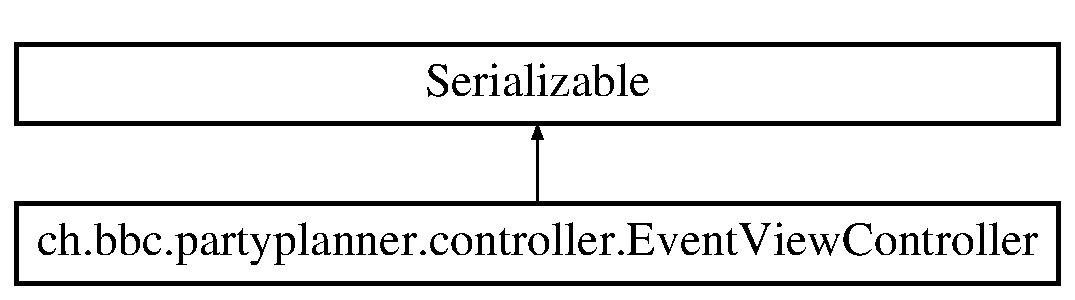
\includegraphics[height=2.000000cm]{classch_1_1bbc_1_1partyplanner_1_1controller_1_1_event_view_controller}
\end{center}
\end{figure}
\subsection*{Public Member Functions}
\begin{DoxyCompactItemize}
\item 
\hypertarget{classch_1_1bbc_1_1partyplanner_1_1controller_1_1_event_view_controller_a5193119c04676995d940407cf54fcae2}{}\label{classch_1_1bbc_1_1partyplanner_1_1controller_1_1_event_view_controller_a5193119c04676995d940407cf54fcae2} 
String {\bfseries get\+Event\+Title} ()
\item 
\hypertarget{classch_1_1bbc_1_1partyplanner_1_1controller_1_1_event_view_controller_ae8351395317f3a7da0d4ff6ac7b73b2f}{}\label{classch_1_1bbc_1_1partyplanner_1_1controller_1_1_event_view_controller_ae8351395317f3a7da0d4ff6ac7b73b2f} 
String {\bfseries bring} ()
\item 
\hypertarget{classch_1_1bbc_1_1partyplanner_1_1controller_1_1_event_view_controller_a590c368ae82b19a25992c8645accdee3}{}\label{classch_1_1bbc_1_1partyplanner_1_1controller_1_1_event_view_controller_a590c368ae82b19a25992c8645accdee3} 
String {\bfseries get\+Event\+Creator} ()
\item 
\hypertarget{classch_1_1bbc_1_1partyplanner_1_1controller_1_1_event_view_controller_af462bacbd7d9f2ed60159f89fc97a86a}{}\label{classch_1_1bbc_1_1partyplanner_1_1controller_1_1_event_view_controller_af462bacbd7d9f2ed60159f89fc97a86a} 
String {\bfseries get\+Event\+Description} ()
\item 
\hypertarget{classch_1_1bbc_1_1partyplanner_1_1controller_1_1_event_view_controller_a5b9a868e05089e7c96afacc640f8661a}{}\label{classch_1_1bbc_1_1partyplanner_1_1controller_1_1_event_view_controller_a5b9a868e05089e7c96afacc640f8661a} 
String {\bfseries get\+Event\+Date} ()
\item 
\hypertarget{classch_1_1bbc_1_1partyplanner_1_1controller_1_1_event_view_controller_a9751b8a8ab45e9510e0962624bafcf71}{}\label{classch_1_1bbc_1_1partyplanner_1_1controller_1_1_event_view_controller_a9751b8a8ab45e9510e0962624bafcf71} 
List$<$ Product $>$ {\bfseries get\+Products} ()
\item 
\hypertarget{classch_1_1bbc_1_1partyplanner_1_1controller_1_1_event_view_controller_aa0bfc4d3def949169f7419805a379840}{}\label{classch_1_1bbc_1_1partyplanner_1_1controller_1_1_event_view_controller_aa0bfc4d3def949169f7419805a379840} 
void {\bfseries set\+Products} (List$<$ Product $>$ all\+Products)
\item 
\hypertarget{classch_1_1bbc_1_1partyplanner_1_1controller_1_1_event_view_controller_a64f445728352ab06ef9eaf4bfd5409db}{}\label{classch_1_1bbc_1_1partyplanner_1_1controller_1_1_event_view_controller_a64f445728352ab06ef9eaf4bfd5409db} 
void {\bfseries init\+Products} ()
\item 
\hypertarget{classch_1_1bbc_1_1partyplanner_1_1controller_1_1_event_view_controller_a3268e78ee60991510aa7e14968a9940a}{}\label{classch_1_1bbc_1_1partyplanner_1_1controller_1_1_event_view_controller_a3268e78ee60991510aa7e14968a9940a} 
int {\bfseries get\+Product\+To\+Delete\+Id} ()
\item 
\hypertarget{classch_1_1bbc_1_1partyplanner_1_1controller_1_1_event_view_controller_a3801fb584bcda970975e1be312f229cb}{}\label{classch_1_1bbc_1_1partyplanner_1_1controller_1_1_event_view_controller_a3801fb584bcda970975e1be312f229cb} 
void {\bfseries set\+Product\+To\+Delete\+Id} (int product\+To\+Delete\+Id)
\item 
\hypertarget{classch_1_1bbc_1_1partyplanner_1_1controller_1_1_event_view_controller_aa3abd7eddc3db459b868f4540e7123e5}{}\label{classch_1_1bbc_1_1partyplanner_1_1controller_1_1_event_view_controller_aa3abd7eddc3db459b868f4540e7123e5} 
int {\bfseries get\+Amount} ()
\item 
\hypertarget{classch_1_1bbc_1_1partyplanner_1_1controller_1_1_event_view_controller_a428dc4421f974d2b46a946f3ea7afdd8}{}\label{classch_1_1bbc_1_1partyplanner_1_1controller_1_1_event_view_controller_a428dc4421f974d2b46a946f3ea7afdd8} 
void {\bfseries set\+Amount} (int amount)
\end{DoxyCompactItemize}


The documentation for this class was generated from the following file\+:\begin{DoxyCompactItemize}
\item 
Event\+View\+Controller.\+java\end{DoxyCompactItemize}

\hypertarget{classch_1_1bbc_1_1partyplanner_1_1controller_1_1_user_controller}{}\section{ch.\+bbc.\+partyplanner.\+controller.\+User\+Controller Class Reference}
\label{classch_1_1bbc_1_1partyplanner_1_1controller_1_1_user_controller}\index{ch.\+bbc.\+partyplanner.\+controller.\+User\+Controller@{ch.\+bbc.\+partyplanner.\+controller.\+User\+Controller}}
Inheritance diagram for ch.\+bbc.\+partyplanner.\+controller.\+User\+Controller\+:\begin{figure}[H]
\begin{center}
\leavevmode
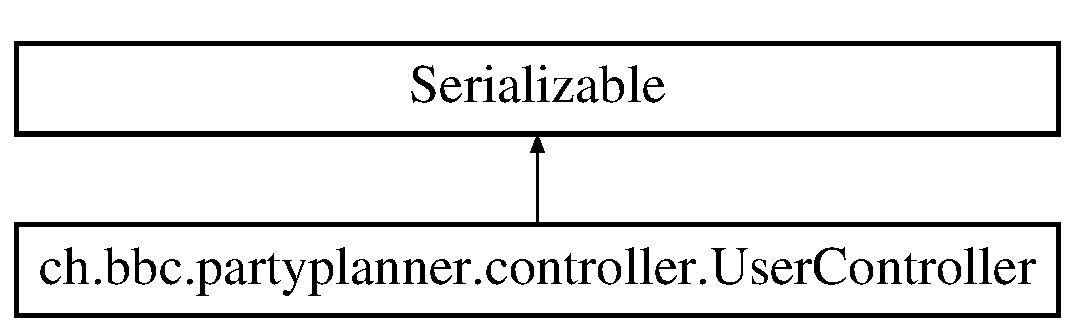
\includegraphics[height=2.000000cm]{classch_1_1bbc_1_1partyplanner_1_1controller_1_1_user_controller}
\end{center}
\end{figure}
\subsection*{Public Member Functions}
\begin{DoxyCompactItemize}
\item 
\hypertarget{classch_1_1bbc_1_1partyplanner_1_1controller_1_1_user_controller_acd2e6cb7c59f69278b81773dcd9d82dc}{}\label{classch_1_1bbc_1_1partyplanner_1_1controller_1_1_user_controller_acd2e6cb7c59f69278b81773dcd9d82dc} 
String {\bfseries create} ()
\item 
\hypertarget{classch_1_1bbc_1_1partyplanner_1_1controller_1_1_user_controller_a2f1a3d9bdfb1ce2e5272e95549aa2926}{}\label{classch_1_1bbc_1_1partyplanner_1_1controller_1_1_user_controller_a2f1a3d9bdfb1ce2e5272e95549aa2926} 
String {\bfseries login} ()
\item 
\hypertarget{classch_1_1bbc_1_1partyplanner_1_1controller_1_1_user_controller_ab0ed3cc99c63ecd241f4675bb59a7824}{}\label{classch_1_1bbc_1_1partyplanner_1_1controller_1_1_user_controller_ab0ed3cc99c63ecd241f4675bb59a7824} 
String {\bfseries logout} ()
\item 
\hypertarget{classch_1_1bbc_1_1partyplanner_1_1controller_1_1_user_controller_a1868f5dda7b160eaef448a2f509c13bf}{}\label{classch_1_1bbc_1_1partyplanner_1_1controller_1_1_user_controller_a1868f5dda7b160eaef448a2f509c13bf} 
int {\bfseries get\+Status} ()
\item 
\hypertarget{classch_1_1bbc_1_1partyplanner_1_1controller_1_1_user_controller_a1ea3d403c763fcc87e53f6fb8715792a}{}\label{classch_1_1bbc_1_1partyplanner_1_1controller_1_1_user_controller_a1ea3d403c763fcc87e53f6fb8715792a} 
void {\bfseries set\+Status} (int status)
\item 
\hypertarget{classch_1_1bbc_1_1partyplanner_1_1controller_1_1_user_controller_a949eb9c3ee0256df9d2a3484e2eacb78}{}\label{classch_1_1bbc_1_1partyplanner_1_1controller_1_1_user_controller_a949eb9c3ee0256df9d2a3484e2eacb78} 
User {\bfseries get\+User} ()
\item 
\hypertarget{classch_1_1bbc_1_1partyplanner_1_1controller_1_1_user_controller_a78816ad412b39dd556723c6d148916f4}{}\label{classch_1_1bbc_1_1partyplanner_1_1controller_1_1_user_controller_a78816ad412b39dd556723c6d148916f4} 
void {\bfseries set\+User} (User user)
\item 
\hypertarget{classch_1_1bbc_1_1partyplanner_1_1controller_1_1_user_controller_adc85fcc9498590a1eca32244a745d852}{}\label{classch_1_1bbc_1_1partyplanner_1_1controller_1_1_user_controller_adc85fcc9498590a1eca32244a745d852} 
List$<$ User $>$ {\bfseries get\+All\+Users} ()
\item 
\hypertarget{classch_1_1bbc_1_1partyplanner_1_1controller_1_1_user_controller_a04bdaad25a2aca511a4837ddc8d43e28}{}\label{classch_1_1bbc_1_1partyplanner_1_1controller_1_1_user_controller_a04bdaad25a2aca511a4837ddc8d43e28} 
void {\bfseries set\+All\+Users} (List$<$ User $>$ all\+Users)
\item 
\hypertarget{classch_1_1bbc_1_1partyplanner_1_1controller_1_1_user_controller_ada4a5cc6843705315fb5d38986e42568}{}\label{classch_1_1bbc_1_1partyplanner_1_1controller_1_1_user_controller_ada4a5cc6843705315fb5d38986e42568} 
boolean {\bfseries is\+User\+Logged\+In} ()
\item 
\hypertarget{classch_1_1bbc_1_1partyplanner_1_1controller_1_1_user_controller_a60f8affd66b54941ca7cd2de282c4c03}{}\label{classch_1_1bbc_1_1partyplanner_1_1controller_1_1_user_controller_a60f8affd66b54941ca7cd2de282c4c03} 
void {\bfseries set\+User\+Logged\+In} (boolean user\+Logged\+In)
\end{DoxyCompactItemize}


The documentation for this class was generated from the following file\+:\begin{DoxyCompactItemize}
\item 
User\+Controller.\+java\end{DoxyCompactItemize}

%--- End generated contents ---

% Index
\backmatter
\newpage
\phantomsection
\clearemptydoublepage
\addcontentsline{toc}{chapter}{Index}
\printindex

\end{document}
